\documentclass[a4paper,10pt]{article}

\usepackage{amssymb,amsmath}
\usepackage[brazilian]{babel}
\usepackage[utf8]{inputenc}
\usepackage{graphicx}
\usepackage{chngcntr}
\usepackage{tikz}
\usepackage{tikz-3dplot}
\usepackage{indentfirst}
\usepackage[numbers,sort&compress]{natbib}
\usepackage[title]{appendix}
\usepackage{subfig}
\usepackage{floatrow}
\usepackage{booktabs}% http://ctan.org/pkg/booktabs
\newcommand{\tabitem}{~~\llap{\textbullet}~~}

\usetikzlibrary{trees}
\usetikzlibrary{decorations.pathmorphing}
\usetikzlibrary{decorations.markings}

\tikzset{
    photon/.style={decorate, decoration={snake}, draw=black},
    fermion/.style={draw=black, postaction={decorate}, 
    decoration={markings,mark=at position .55 with {\arrow[scale=2,draw=black]{>}}}},
    afermion/.style={draw=black, postaction={decorate}, 
    decoration={markings,mark=at position .55 with {\arrow[scale=2,draw=black]{<}}}},
    gluon/.style={decorate, draw=green,
    decoration={coil,amplitude=4pt, segment length=5pt}} 
    }

\counterwithin{figure}{subsection}

\usepackage{afterpage}

\newcommand\blankpage{%
    \null
    \thispagestyle{empty}%
    \addtocounter{page}{-1}%
    \newpage}
    
\setlength{\parindent}{20pt}


%opening
\title{Notas em QGP}
\author{Fabio de Moraes Canedo}

\begin{document}

\maketitle

\begin{abstract}
Resumo das minhas notas no estudo de Íons Pesados.
\end{abstract}

\section{Instrodução}



\subsection{Plasma de Quarks e Gluons}

\ \ Em colisões íons pesados, ou seja, íons com número de massa da ordem de $10^2$, a uma energia da ordem de $10^2 GeV$,
uma quantidade considerável de energia é depositada na região de interação. Essa nergia, na forma de quarks e gluons,
libera novos graus de liberdade, realizando uma transição de fase para um estado da matéria conhecido como Plasma de Quarks e Gluons(QGP,
sigla em inglês).
\par
A temperatura necessária para formar este estado da matéria é da ordem de centenas de $MeV$ ou
$10^{12} K$, cerca de $10$ mil vezes a temperatura do centro do Sol, e a densidade de energia é da ordem de $0.2-1
GeV/fm^{3}$. As propriedades deste estado da matéria podem ser estudadas analisando os produtos dessa colisão após o resfriamento
da matéria. O espectro de $p_T$\footnote{Ver seção \ref{variaveis}} das partículas, por exemplo, fornece insformações sobre a entropia
e a temperatura do plasma, através da multiplicidade e da inclinação do gráfico, respectivamente. Em geral, essas propriedades estarão
associadas ao espectro na faixa de $p_T \approx 0-2 GeV/c$. Na faixa $p_T > 2 GeV/c$, observa-se os efeitos de fenômenos
da classe {\it hard scaterring}. Estes fenômenos são resultados da formação de partículas de alta energia que atravessam o plasma
aquecido, depositando energia neste. Na sua saída, devido às propriedades da QCD\footnote{QCD ou {\it Quantum Chromodynamics} é a 
teoria que descreve as interações fortes.}, essas partículas se fragmentam criando os chamados {\it jets}.





\subsection{Rapidity} \label{variaveis}

Uma variável útil de se definir em um estudo de colisões de partículas a velocidades relativísticas é a {\it rapidity} $y$. Mas antes,
definimos o conceito de massa transversa.
\par
Toda colisão de partículas possui um eixo específico, chamdo eixo de colisão. Associado a este eixo, há um plano transverso. As componentes
dos momentos no eixo da colisão e no plano transverso serão identificadas como $p_{L}$ e $p_{T}$, respectivamente. Essas variáveis podem ser
melhor compreendidas observando a Figura \ref{fig:geometria}.

\begin{figure}[!h]
 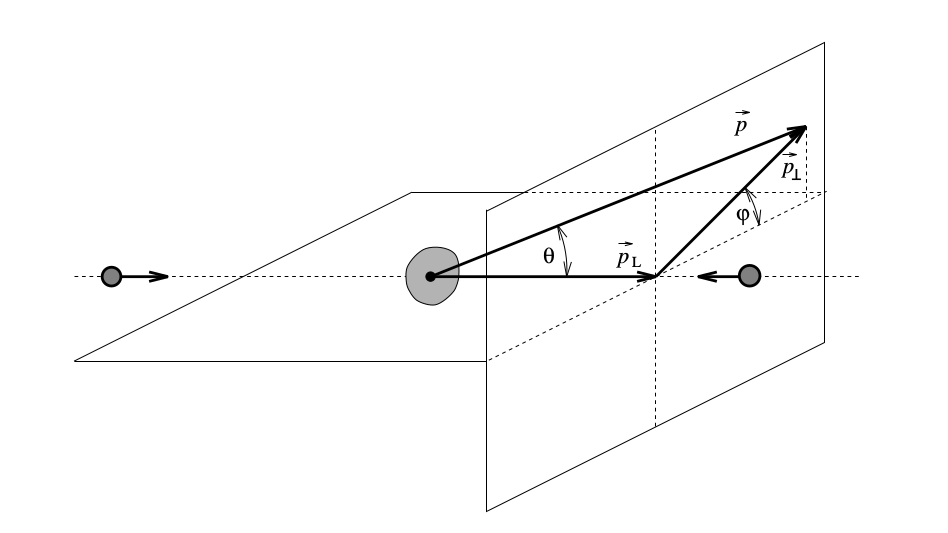
\includegraphics[scale=0.35]{Introducao/geometriamomento.png}
 \caption{Ilustração geométrica de $p_T$ e $p_L$.}
 \label{fig:geometria}
\end{figure}


Associada ao momento transversal, definimos a massa transversa:

\begin{equation}
 m_{T}=\sqrt{m^2+p_{T}^2}
\end{equation}

Ao contrário de $p_{L}$, $p_{T}$ não depende do referencial em que a colisão é estudada, portando, é uma boa variável. É necessário, então,
definir uma variável no eixo de colisão, esta será a {\it rapidity}. Definimos esta através das equações:

\begin{subequations}
\begin{align}
 E=m_{T} \cosh{(y)} \\ p_{L}=m_{T} \sinh{(y)}
\end{align}
\end{subequations}

Isolando $\eta$ nas equações acima obtemos:

\begin{equation}
 y = \ln{(\frac{E+p_{L}}{m_{T}})}
\end{equation}

Uma propriedade importante desta variável, é que ela é aditiva em relação a transformações de Lorentz.

\subsection{Pseudorapidity}

Quando a energia de uma partícula é muito grande comparada à sua massa, podemos escrever:

\begin{equation}
\begin{split}
 y   & = \ln{\frac{E+p_{L}}{m_{T}}} \\
     & = \frac{1}{2}\ln{\frac{(E+p_{L})^2}{m_{T}^2}} \\
     & = \frac{1}{2}\ln{\frac{(E+p_{L})^2}{E^2-p_{L}^2}} \\
     & = \frac{1}{2}\ln{\frac{E+p_{L}}{E-p_{L}}} \\
     & \approx \frac{1}{2}\ln{\frac{p+p_{L}}{p-p_{L}}} \\
     & \approx \frac{1}{2}\ln{\frac{1+\cos(\theta)}{1-\cos(\theta)}} \\
     & \approx \frac{1}{2}\ln{\cot{2\theta}} \\
\end{split}
\end{equation}

Definimos então, a variável {\it pseudorapidity}:

\begin{equation}
 \eta = \frac{1}{2}\ln{\cot{2\theta}}
\end{equation}



\subsection{Modelo de Glauber}\label{glauber}

Sempre que estudamos colisões de íons pesados, é necessário fornecer as condições iniciais da colisão. O modelo
de Glauber baseia-se na ideia de que os nucleons pertencentes ao núcleo projétil realizam colisões dois a dois seguindo trajetórias
retas atravessando o núcleo alvo. A distribuição dos nucleons nos dois núcleos, tanto alvo quanto o projétil, seguem a distribuição de
Woods-Saxon:

\begin{equation}
 \rho(r) = \frac{\rho_0}{1+\exp{(\frac{r-R}{a})}}
\end{equation}

Normalmente, os núcleons são gerados em uma distribuição espacial que obedece tal distribuição, em seguida, sua trajetória
é traçada em linha reta, considerando colisões com todos os núcleons em seu caminho. Uma descrição detalhada deste modelo e a
geração de condições iniciais pode ser encontrada em \cite{miller_glauber_2007}.

\subsection{Algoritmos de Reconstrução de Jatos}

Para realizar a reconstrução de jatos\cite{salam_towards_2010}, costuma-se definir a seguinte quantidade:

\begin{equation}
 \Delta R_{ij} = \sqrt{(\eta_i-\eta_j)^2+(\phi_i-\phi_j)^2}
\end{equation}

Essa será, para as duas partículas, aqui chamadas de $i$ e $j$, uma distância angular
definida entre as duas. A maioria dos algoritmos de jatos irão utilizar essa definição de distância angular para realizar os agrupamentos,
ou {\it clusters} de partículas para a reconstrução dos jatos. Estes são chamados os algoritmos de cones. Um algoritmo
comumente utilizado consiste em, primeiro definir um parâmetro $R$, em seguida, escolher uma partícula {\it semente}, normalmente, escolhe-se
a partícula de maor $p_T$. Após esses passos, localizamos a partícula de maior $p_T$ a uma distância menor ou igual a $R$.
\par
Então, retiramos essas duas partículas dos dados e definimos uma nova partícula com momento:

\begin{equation}
 p_{\mu}^{J} = p_{\mu}^1 + p_{\mu}^2
\end{equation}

Essa partícula define o novo centro do cone, agora procuramos a partícula de maior $p_T$ de distância menor ou igual a $R$ desta, e assim por
diante.


\subsection{Efeitos Anisotrópicos do {\it Jet Quenching}} \label{ef_an}

Ao atravessar a matéria densa e quente, o parton perde energia e se resfria. A energia perdida
por este é depositada na matéria densa e quente, afetando a expansão hidrodinâmica do QGP
\cite{andrade_jet_2014}. Podemos observar estes efeitos na Figura \ref{fig:v2}.

\begin{figure}[!htb]
\centering
 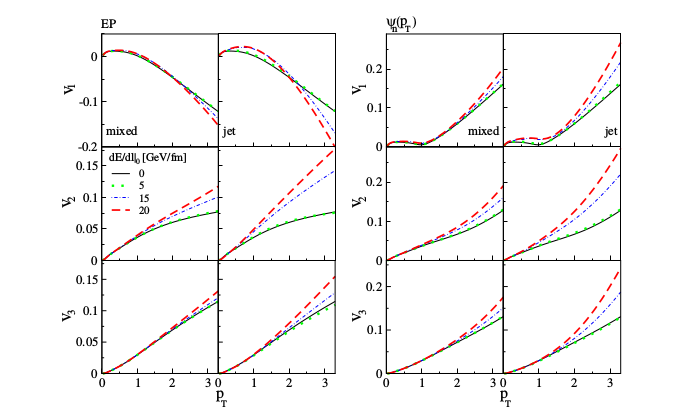
\includegraphics[scale=0.4]{Introducao/v2.png}
 \caption{Efeitos dos Jatos nos Harmônicos para diferentes valores de $p_{T}$.}
 \label{fig:v2}
\end{figure}

O estudo foi realizado basicamente com a inserão de um termo fonte nas equações hidrodinâmicas, da seguinte maneira:

\begin{equation}
 \partial_{\mu} T^{\mu \nu} = J^{\nu}
\end{equation}

O termo fonte foi construído conforme a equação:

\begin{equation}
 J^{\nu}(\tau,\overrightarrow{r}) = \sum_{n=1}^{n_p} \frac{s(\overrightarrow{r}^{jet}_{n}(\tau))}{s_0} \frac{dE}{dl}\bigg|_0
 F(\overrightarrow{r}-\overrightarrow{r}^{jet}_{n}(\tau),\tau;\sigma)(1,\overrightarrow{v}^{jet}_{n},0)
\end{equation}

A soma em questão é realizada sobre os partons viajando pela matéria densa. Os termos $s(\overrightarrow{r}^{jet}_{n}(\tau))$ e $s_0$
correspondem às entropias calculadas na posição do parton e em uma entropia de referência, respectivamente. A função $F$ corresponde a uma
distribuição Gaussiana representando o alcance do efeito do parton. E $\overrightarrow{v}^{jet}_{n}$ representa a velocidade do n-ésimo
parton.
\blankpage

\section{Métodos}

\subsection{MUSIC}

O programa MUSIC, a ser utilizado nas simulações deste trabalho, é um
gerador de eventos que pode ser encontrado em \cite{noauthor_music_nodate}.
\par
Em \cite{schenke_3+1d_2010} encontramos uma descrião mais detalhada do algoritmo empregado. Alguns fatos
são citados a seguir:

\begin{itemize}
 \item O método KURGANOV-TADMOR é implementado, este método baseia-se na introdução de
 um termo de dissipação numérica para garantia de estabilidade, é capaz de lidar com
 choques e descontinuidades, ideal para a inserção de termos fonte como deposição de energia
 de jatos;
 \item As condições iniciais são baseadas no modelo de Glauber e na parametrização de Woods-Saxon,
 ver subseção \ref{glauber};
 \item Uma simplificação das equações é atingida escolhendo variáveis através de uma rotação hiperbólica;
 \item O {\it freeze-out} é construído assumindo a fórmula de Cooper-Frye\cite{teaney_chemical_2002};
\end{itemize}

É interessante observar na Figura \ref{fig:musicv2} que o MUSIC não fornece resultados coerentes com os experimentos na faixa de $p_T$
entre $1$ e $2 GeV$. Isso poderia ser explicado pela ausência de energia depositada pelos jatos, que incluem na hidrodinâmica efeitos
anisotrópicos\cite{andrade_jet_2014}, ver Figura \ref{fig:v2}.

\begin{figure}[!h]
\centering
 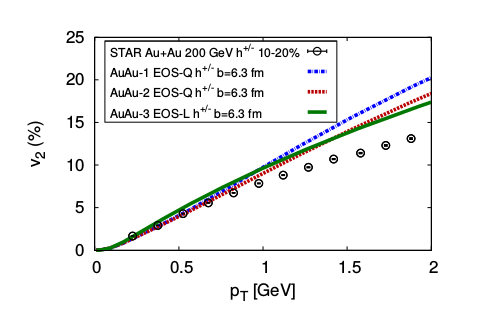
\includegraphics[scale=0.5]{Metodos/music_results.png}
 \caption{Resultados do MUSIC no coeficiente $V_{2}$.}
 \label{fig:musicv2}
\end{figure}


\bibliography{Bibliografia/bibliografia} 
\bibliographystyle{ieeetr}

\end{document}
\grid
\grid
